\documentclass[11pt,a4paper]{report} 
% Alternativ für doppelseitigen Ausdruck (nur bei > 60 Seiten sinnvoll)
%\documentclass[11pt,a4paper,twoside,openright]{report} 

% Deutsch
\usepackage[german]{babel} % deutsch und deutsche Rechtschreibung
\usepackage[utf8]{inputenc} % Unicode Text 
\usepackage[T1]{fontenc} % Umlaute und deutsches Trennen
\usepackage{textcomp} % Euro
\usepackage[hyphens]{url}
% statt immer Ab\-schluss\-ar\-beit zu schreiben
% einfach hier sammeln mit -. 
\hyphenation{Ab-schluss-ar-beit}
% Vorsicht bei Umlauten und Bindestrichen
\hyphenation{Ver-st\"ar-ker-aus-gang}
 % eigene Hyphenations, die für das Dokument gelten
\usepackage{amssymb} % Symbole
\usepackage{enumitem}
\usepackage{tabularx}


%% Fonts, ein kompletter Satz an Optionen
% Times New Roman, gewohnter Font mit ok tt und serifenlos
%\usepackage{mathptmx} 
%\usepackage[scaled=.95]{helvet}
%\usepackage{courier}
% Palatino, mal was anderes, auch mit ok tt und serifenlos
% empfohlen
\usepackage{mathpazo} % Palatino, mal was anderes
\usepackage[scaled=.95]{helvet}
\usepackage{courier}
% New Century Schoolbook sieht auch nett aus (macht auch tt und serifenlos)
%\usepackage{newcent}

% zusätzlich: Default serifenlos mit Helvetica 
% ich kann es nicht mehr sehen...
%\renewcommand{\familydefault}{\sfdefault}

\usepackage{microtype}

% Bilder und Listings
\usepackage{graphicx} % wir wollen Bilder einfügen
\usepackage{subfig} % Teilbilder
\usepackage{wrapfig} % vielleicht doch besser vermeiden
\usepackage{listings} % schöne Quellcode-Listings
% ein paar Einstellungen für akzeptable Listings
\lstset{basicstyle=\sffamily, columns=[l]flexible, mathescape=true, showstringspaces=false, numbers=left, numberstyle=\tiny}
\lstset{language=python} % und nur schöne Programmiersprachen ;-)
% und eine eigene Umgebung für Listings
\usepackage{float}
\newfloat{listing}{htbp}{scl}[chapter]
\floatname{listing}{Listing}

% Seitenlayout
%\usepackage[paper=a4paper,width=14cm,left=35mm,height=22cm]{geometry}
\usepackage[paper=a4paper,width=14cm,height=22cm]{geometry}
\usepackage{setspace}
\linespread{1.15}
\setlength{\parskip}{0.5em}
\setlength{\parindent}{0em} % im Deutschen Einrückung nicht üblich, leider

% Seitenmarkierungen 
\newcommand{\phv}{\fontfamily{phv}\fontseries{m}\fontsize{9}{11}\selectfont}
\usepackage{fancyhdr} % Schickere Header und Footer

\pagestyle{fancy}
\renewcommand{\chaptermark}[1]{\markboth{#1}{}}
\renewcommand{\sectionmark}[1]{\markright{#1}}
\fancyhead[LO]{\phv \nouppercase{\leftmark}}
\fancyhead[RE]{\phv \nouppercase{\rightmark}}
\fancyhead[RO,LE]{\phv \thepage}
\fancyfoot[C]{\ } % Seitenzahl unten nur Kapitel


% Theorem-Umgebungen
\newtheorem{definition}{Definition}[chapter]
\newtheorem{satz}{Satz}[chapter]
\newtheorem{lemma}[satz]{Lemma} % gleicher Zähler wie Satz
\newtheorem{theorem}{Theorem}[chapter]
\newenvironment{beweis}[1][Beweis]{\begin{trivlist}
\item[\hskip \labelsep {\textit{#1 }}]}{\end{trivlist}}
\newcommand{\qed}{\hfill \ensuremath{\square}}

% Inhaltsverzeichnis
\setcounter{tocdepth}{1}
\setcounter{secnumdepth}{2}

% Quellen teilen
\usepackage{bibtopic} 

% Hochschule Logo, noch nicht perfekt
\usepackage{hsrmlogo}

% Spezialpakete
\usepackage{epigraph}
\setlength{\epigraphrule}{0pt} % kein Trennstrich

% damit wir nicht so viel tippen müssen, nur für Demo 
\usepackage{blindtext} 

% Zum Zeigen von Fehlern
\usepackage{soul}
\newcommand*\falsch{\st}

% Links im PDF
\usepackage{hyperref}
\hypersetup{
    colorlinks=true,
    citecolor=black,
    filecolor=black,
    linkcolor=black,
    urlcolor=black
}

% Kommentare
\usepackage{comment} % alle Pakete und Einstellungen	
\usepackage{hyperref}
% Hier anpassen 
\newcommand{\titel}{Entwurf, prototypische Implementierung und Evaluation eines Sicherheitskonzepts für die Authentifizierung und Autorisierung von Fernzugriffen auf eine Automatisierungsanlage}
\newcommand{\kurztitel}{Template Abschlussarbeit}
\newcommand{\autor}{Kevin Sapper}
\newcommand{\datum}{09. Oktober 2014} % Abgabedatum
\newcommand{\ort}{Wiesbaden}
\newcommand{\referent}{Prof.\ Dr.\ Reinhold Kröger}
\newcommand{\korreferent}{Prof.\ Dr.\ Martin Gergeleit}

\begin{document}
\pagenumbering{Roman}

\begin{titlepage}
  \begin{center}
    % Kopf der Seite
    \hsrmlogo[1]
    \parbox[b]{8cm}{Hochschule RheinMain \\
     Fachbereich Design Informatik Medien \\
     Studiengang Angewandte Informatik}
    \vfill    
    {\LARGE Abschlussarbeit} \\[0.5cm]
    {\large zur Erlangung des akademischen Grades} \\[5mm]
    {\large Bachelor of Science (B.Sc.)} \\[5mm]
    \rule{\textwidth}{1pt}\\[0.5cm]
    {\begin{spacing}{1.15} \huge \bfseries \titel \\ \end{spacing}}
    \rule{\textwidth}{1pt}    
    \vfill    
    \begin{tabular}{ll} % Mitte der Seite
      Vorgelegt von & \autor \\
      am & \datum \\
      Referent & \referent \\
      Korreferent & \korreferent
    \end{tabular}    
    \vfill
  \end{center}
\end{titlepage}
\cleardoublepage


% Erklärung gemäß den Allgemeinen Bestimmungen für Prüfungsordnungen
% der Paragraph schwankt, daher ohne Nennung einer Nummer
\section*{Erklärung gemäß ABPO}
\thispagestyle{empty}
Ich erkläre hiermit,
\begin{itemize}
\item dass ich die vorliegende Abschlussarbeit selbstständig angefertigt,
\item keine anderen als die angegebenen Quellen benutzt,
\item die wörtlich oder dem Inhalt nach aus fremden Arbeiten entnommenen 
  Stellen, bildlichen Darstellungen und dergleichen als solche genau 
  kenntlich gemacht und
\item keine unerlaubte fremde Hilfe in Anspruch genommen habe.
\end{itemize}

\vspace{6em}
\noindent\begin{tabular}{p{0.37\textwidth}p{0.56\textwidth}}
\ort, \datum  & \rule{0.56\textwidth}{0.5pt}\\
              & \makebox[1cm]{\ } \autor
\end{tabular}

\vfill

\section*{Erklärung zur Verwendung der Bachelor Thesis}

Hiermit erkläre ich mein Einverständnis mit den im folgenden 
aufgeführten Verbreitungsformen dieser Abschlussarbeit:

\vspace{1em}
\noindent\begin{tabular}{|p{0.82\textwidth}|c|c|}
  \hline
  \textbf{Verbreitungsform} & \makebox[0.035\textwidth]{\textbf{Ja}} 
                            & \makebox[0.05\textwidth]{\textbf{Nein}} \\\hline
  Einstellung der Arbeit in die Hochschulbibliothek 
                         mit Datenträger   &  & $\times$ \\\hline
  Einstellung der Arbeit in die Hochschulbibliothek  
                         ohne Datenträger  & $\times$ & \\\hline
  Veröffentlichung des Titels der Arbeit im Internet  
                                           & $\times$ & \\\hline
  Veröffentlichung der Arbeit im Internet             
                                           & $\times$ & \\\hline
\end{tabular}

\vspace{6em}
\noindent\begin{tabular}{p{0.37\textwidth}p{0.56\textwidth}}
\ort, \datum  & \rule{0.56\textwidth}{0.5pt}\\
              & \makebox[1cm]{\ } \autor
\end{tabular}
\cleardoublepage

 % Titelseite, Erklärungen, etc.

\begin{comment}
\begin{abstract} 
\end{abstract}
\epigraphhead[70]{\epigraph{The user's going to pick dancing pigs over security every time.}{\textit{Bruce Schneier}}}
\epigraphhead[70]{\epigraph{Companies spend millions of dollars on firewalls, encryption and secure access devices, and it’s money wasted, because none of these measures address the weakest link in the security chain.}{\textit{Kevin Mitnick}}}
\epigraphhead[70]{\epigraph{Wisdom consists in being able to distinguish among dangers and make a choice of the least harmful.}{\textit{Niccolo Machiavelli, The Prince}}}
\epigraphhead[70]{\epigraph{Using encryption on the Internet is the equivalent of arranging an armored car to deliver credit card information from someone living in a cardboard box to someone living on a park bench.}{\textit{Gene Spafford}}}
\end{comment}

\tableofcontents
\clearpage 

\pagenumbering{arabic}

\chapter{Einführung} \label{chap:intro}

\begin{itemize}
\item Entwurf -- CATWOE soft systems methodology (SSM)
\item Sicherheitskonzept
\item Authentifizerung \& Autorisierung
\item Fernzugriff
\item Automatisierungsanlage
\item Evaluation
\item prototypische Implementierung
\end{itemize}
 
Im Bereich Kältetechnik wird Regelungstechnik zur Vernetzung und Überwachung von Kälteanlagen entwickelt. Hierzu gehören die Produkte aus der E*LDS Reihe. Diese beinhalten Verbundsteuerungen zur Kälteerzeugung, Kühlstellenregler zur temperaturgenauen Reglung aller Arten von Kühlmöbeln und Kühlräumen, Funk-Temperatursensoren und der Marktrechner als zentrale Intelligenz einer Kälteanlage.

\chapter{Bedrohungsmodell} \label{chap:threat}
\epigraphhead[70]{\epigraph{The only truly secure system is one that is powered off, cast in a block of concrete and sealed in a lead-lined room with armed guards.}{\textit{Gene Spafford}}}

%\begin{figure}[h]
\begin{wrapfigure}{r}{6cm}
\centering
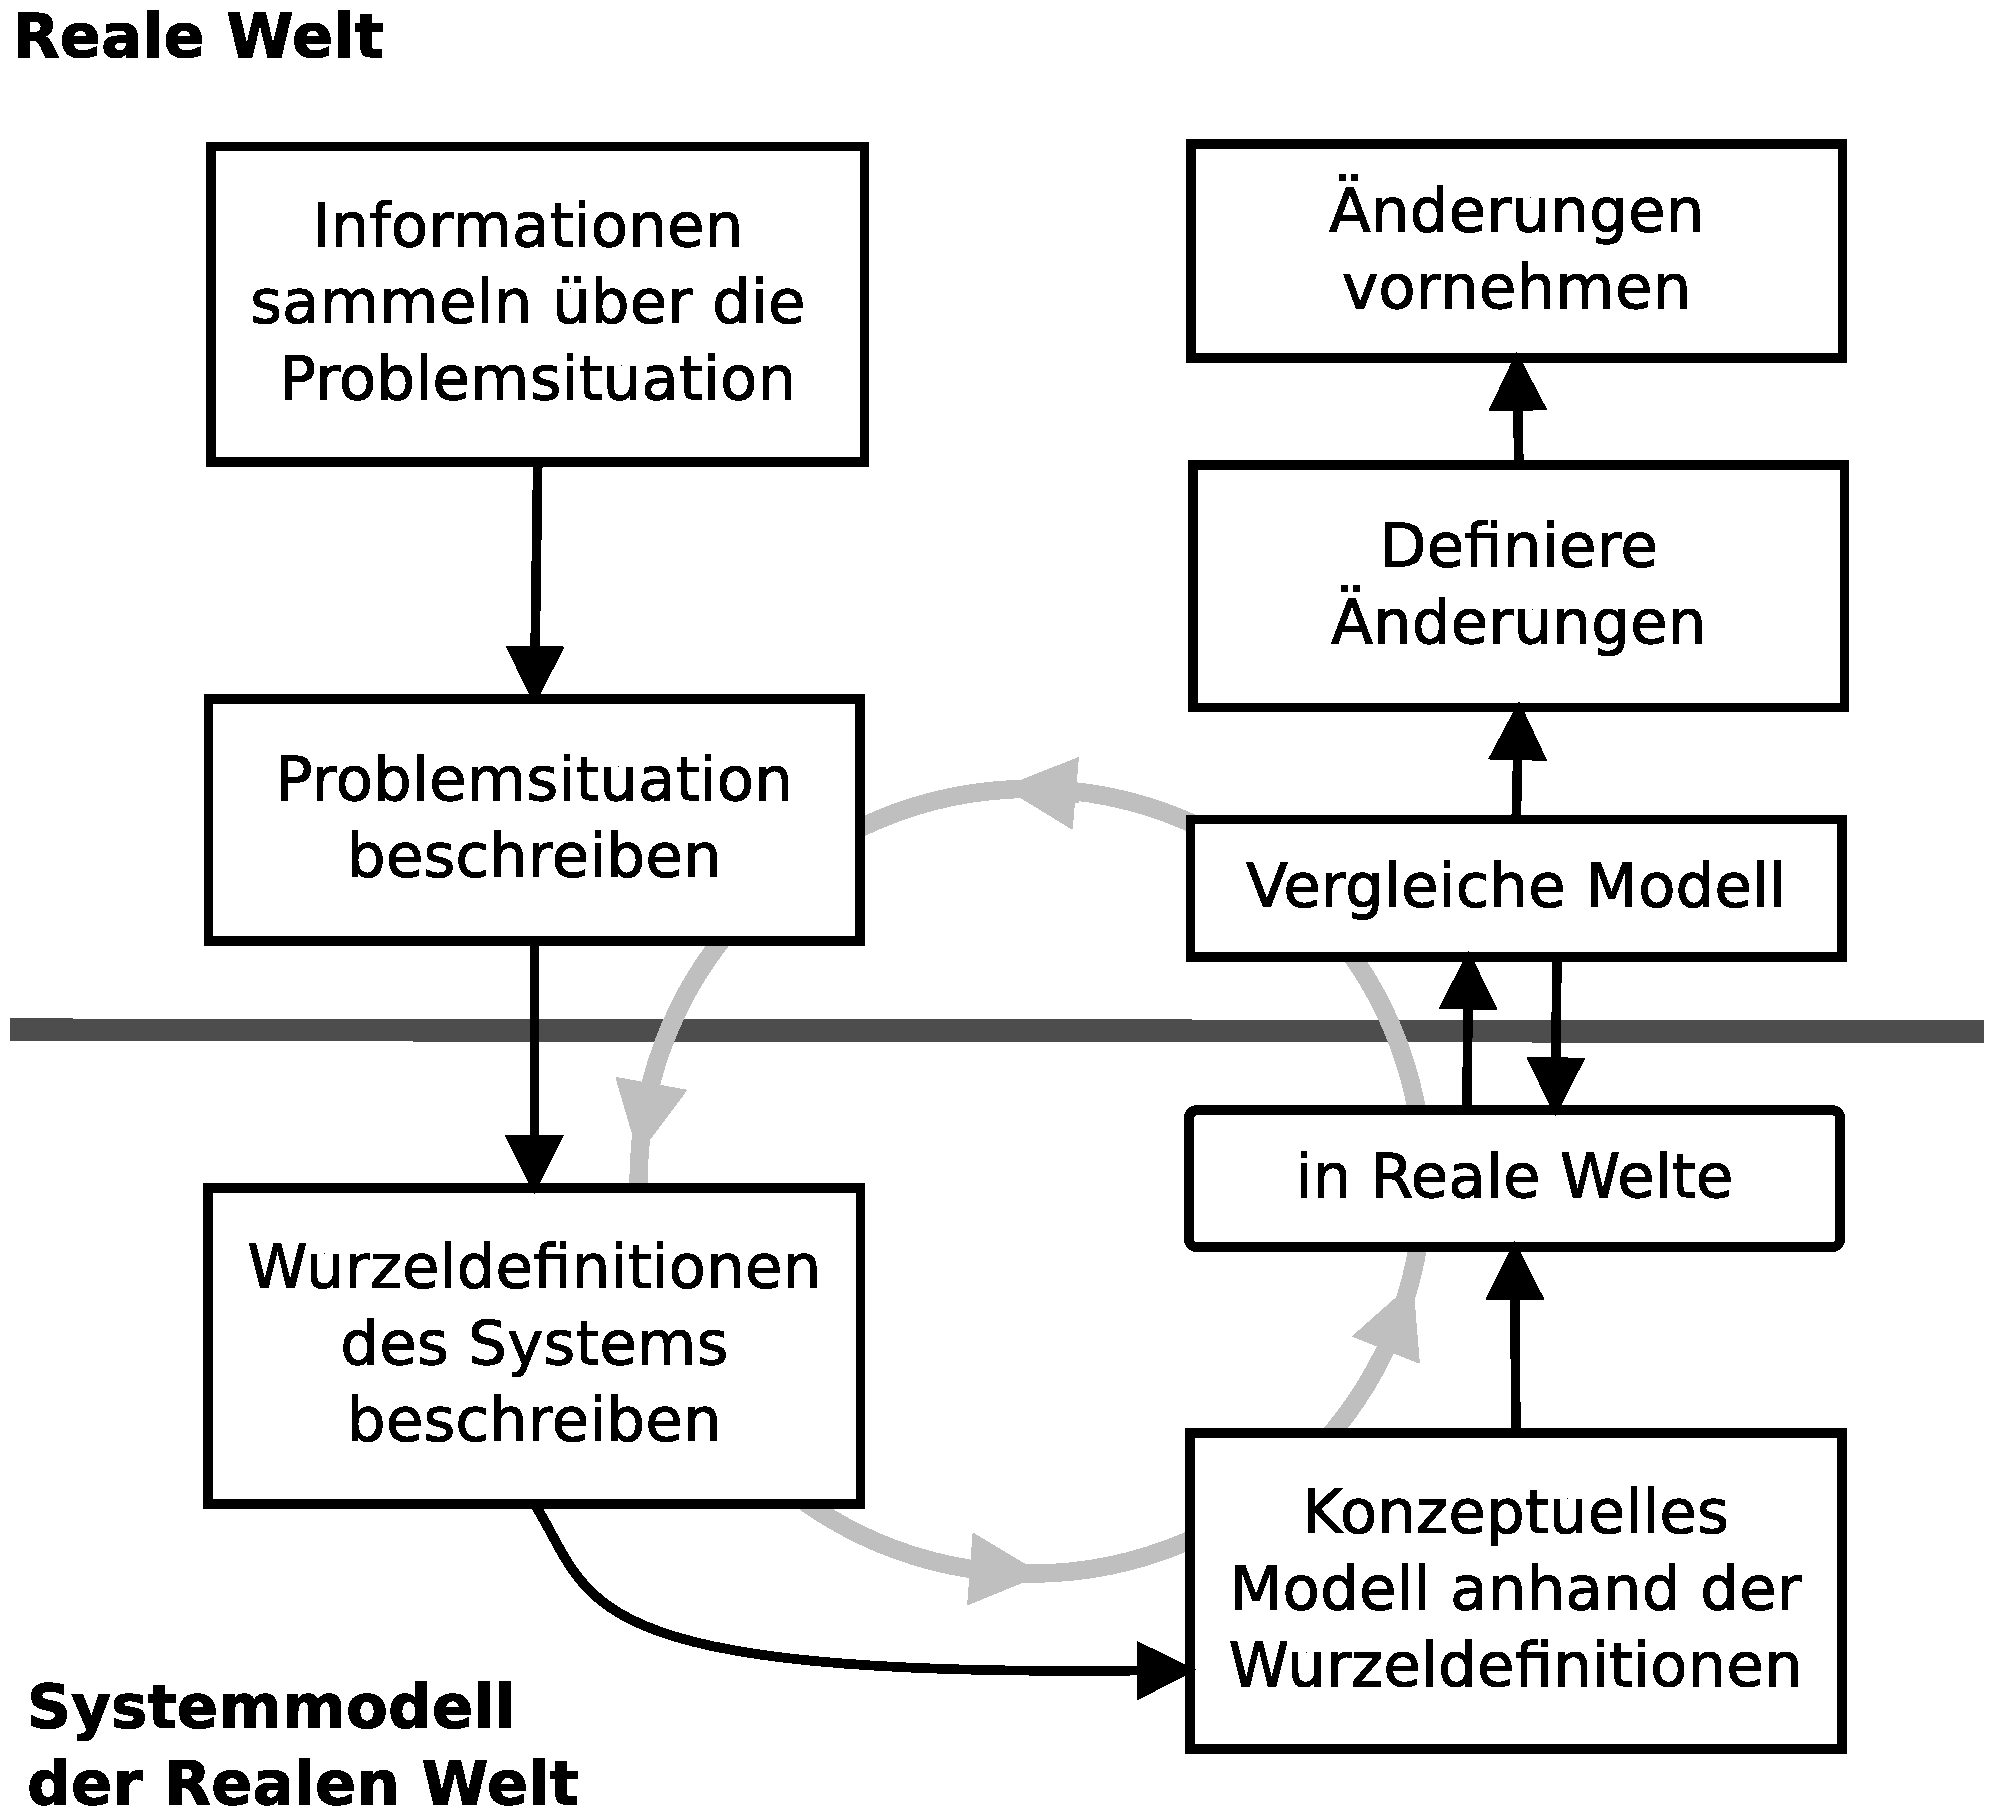
\includegraphics[width=6cm]{images/ssm.pdf}
\caption{Soft Systems Methodologie}
\label{fig:ssm}
\end{wrapfigure}
%\end{figure}

Das Bedrohungsmodell soll auf mögliche Gefahren des aktuellen Systems hinweisen und diese schrittweise, durch geeignete Maßnahmen, eindämmen. Eine geeignete Analyse- und Designmethodik hierfür, bietet die Soft Systems Methodology (SSM), Abbildung~\ref{fig:ssm}. Diese legt besonderes Augenmerk auf die Trennung von Realer Welt und Systemmodell der Realen Welt. In der ersten Phase soll die gesamte Problemsituation, aus Sicht aller Beteiligten, erörtert und unstrukturiert beschrieben werden. Anhand dieser Informationen werden, für das Systemmodell der Realen Welt, Problem- und Zieldefinition festgelegt. Um ein möglichst komplettes Bild der Bedrohung zu bekommen, werden die Definitionen aus der Sicht eines Verteidigers und der Sicht eines Angreifers beleuchtet. Dadurch entstehen zwei konzeptionelles Modelle. Diese werden anschließend gegen die reale Welt und gegeneinander verglichen. Da eine Lösung in erster Iteration meist nicht erzielt wird, können die Vorgänge beliebig wiederholt werden. Wenn der Prozess abgeschlossen ist muss zum Schluss eine Menge an Änderungen festgelegt werden, welche vorgenommen werden sollen.

\section{Problemfeld} \label{sec:problemfeld}

Betrachtet man eine Kälteanlage, dann ist der Marktrechner ihr Herzstück. Über das Bussystem Controller Area Network (CAN) ist er mit sämtlichen Komponenten der Anlage verbunden. Darüber ist in der Lage, Komponenten zentral zu parametrieren und zu überwachen. Sämtliche Betriebsdaten und Betriebszustände, Meldungen und Alarme aus der Überwachung werden, auf seinem internen Speicher, archiviert. Viele Kälteanlagen benötigen viele Meter Leitungen, um die Leitungslänge zu optimieren werden die Meisten in Lowspeed betrieben. Dies erhöht zwar die mögliche Leitungslänge, senkt allerdings die Datenrate auf 125 kbit/s. Bei dieser Datenrate ist die maximale Teilnehmeranzahl auf ca. 100 begrenzt. Die 24-Stunden Überwachung vor Ort durch einen Mitarbeiter ist bei der Menge an Anlagen nicht wirtschaftlich. Deshalb werden heutzutage Fernservice-Zentralen eingesetzt. Aktuell sind Fernservice-Zentralen über VPN mit einem oder mehreren Unternehmensnetzwerken, ihrer Kunden, verbunden. Über dieses können die Marktrechner erreicht werden. Auf diese Weise kann eine einzige Fernservice-Zentrale Tausende Marktrechner überwachen. Tritt ein Fehler auf, kann die Fernservice-Zentrale entweder direkt eingreifen oder einen Monteur zum betreffenden Kunden schicken, der die Anlage instand setzt.

\begin{comment}
@startuml images/problemfeld.svg
skinparam monochrome true
skinparam dpi 150

package "Unternehmensnetzwerk A" as UA {
  [Marktrechner 1]
  [Marktrechner 2]
  [...]
  [Marktrechner n]
}

package "Unternehmensnetzwerk B" as UB {
}

package "Unternehmensnetzwerk C" as UC {
}

cloud VPN {
}

[Fernservice-Zentrale] -down- VPN
VPN -down- UA
VPN -left- UB
VPN -right- UC
UA - [Marktrechner n]
UA - [...]
UA - [Marktrechner 2]
UA - [Marktrechner 1]

@enduml
\end{comment}

\begin{figure}[h]
\centering
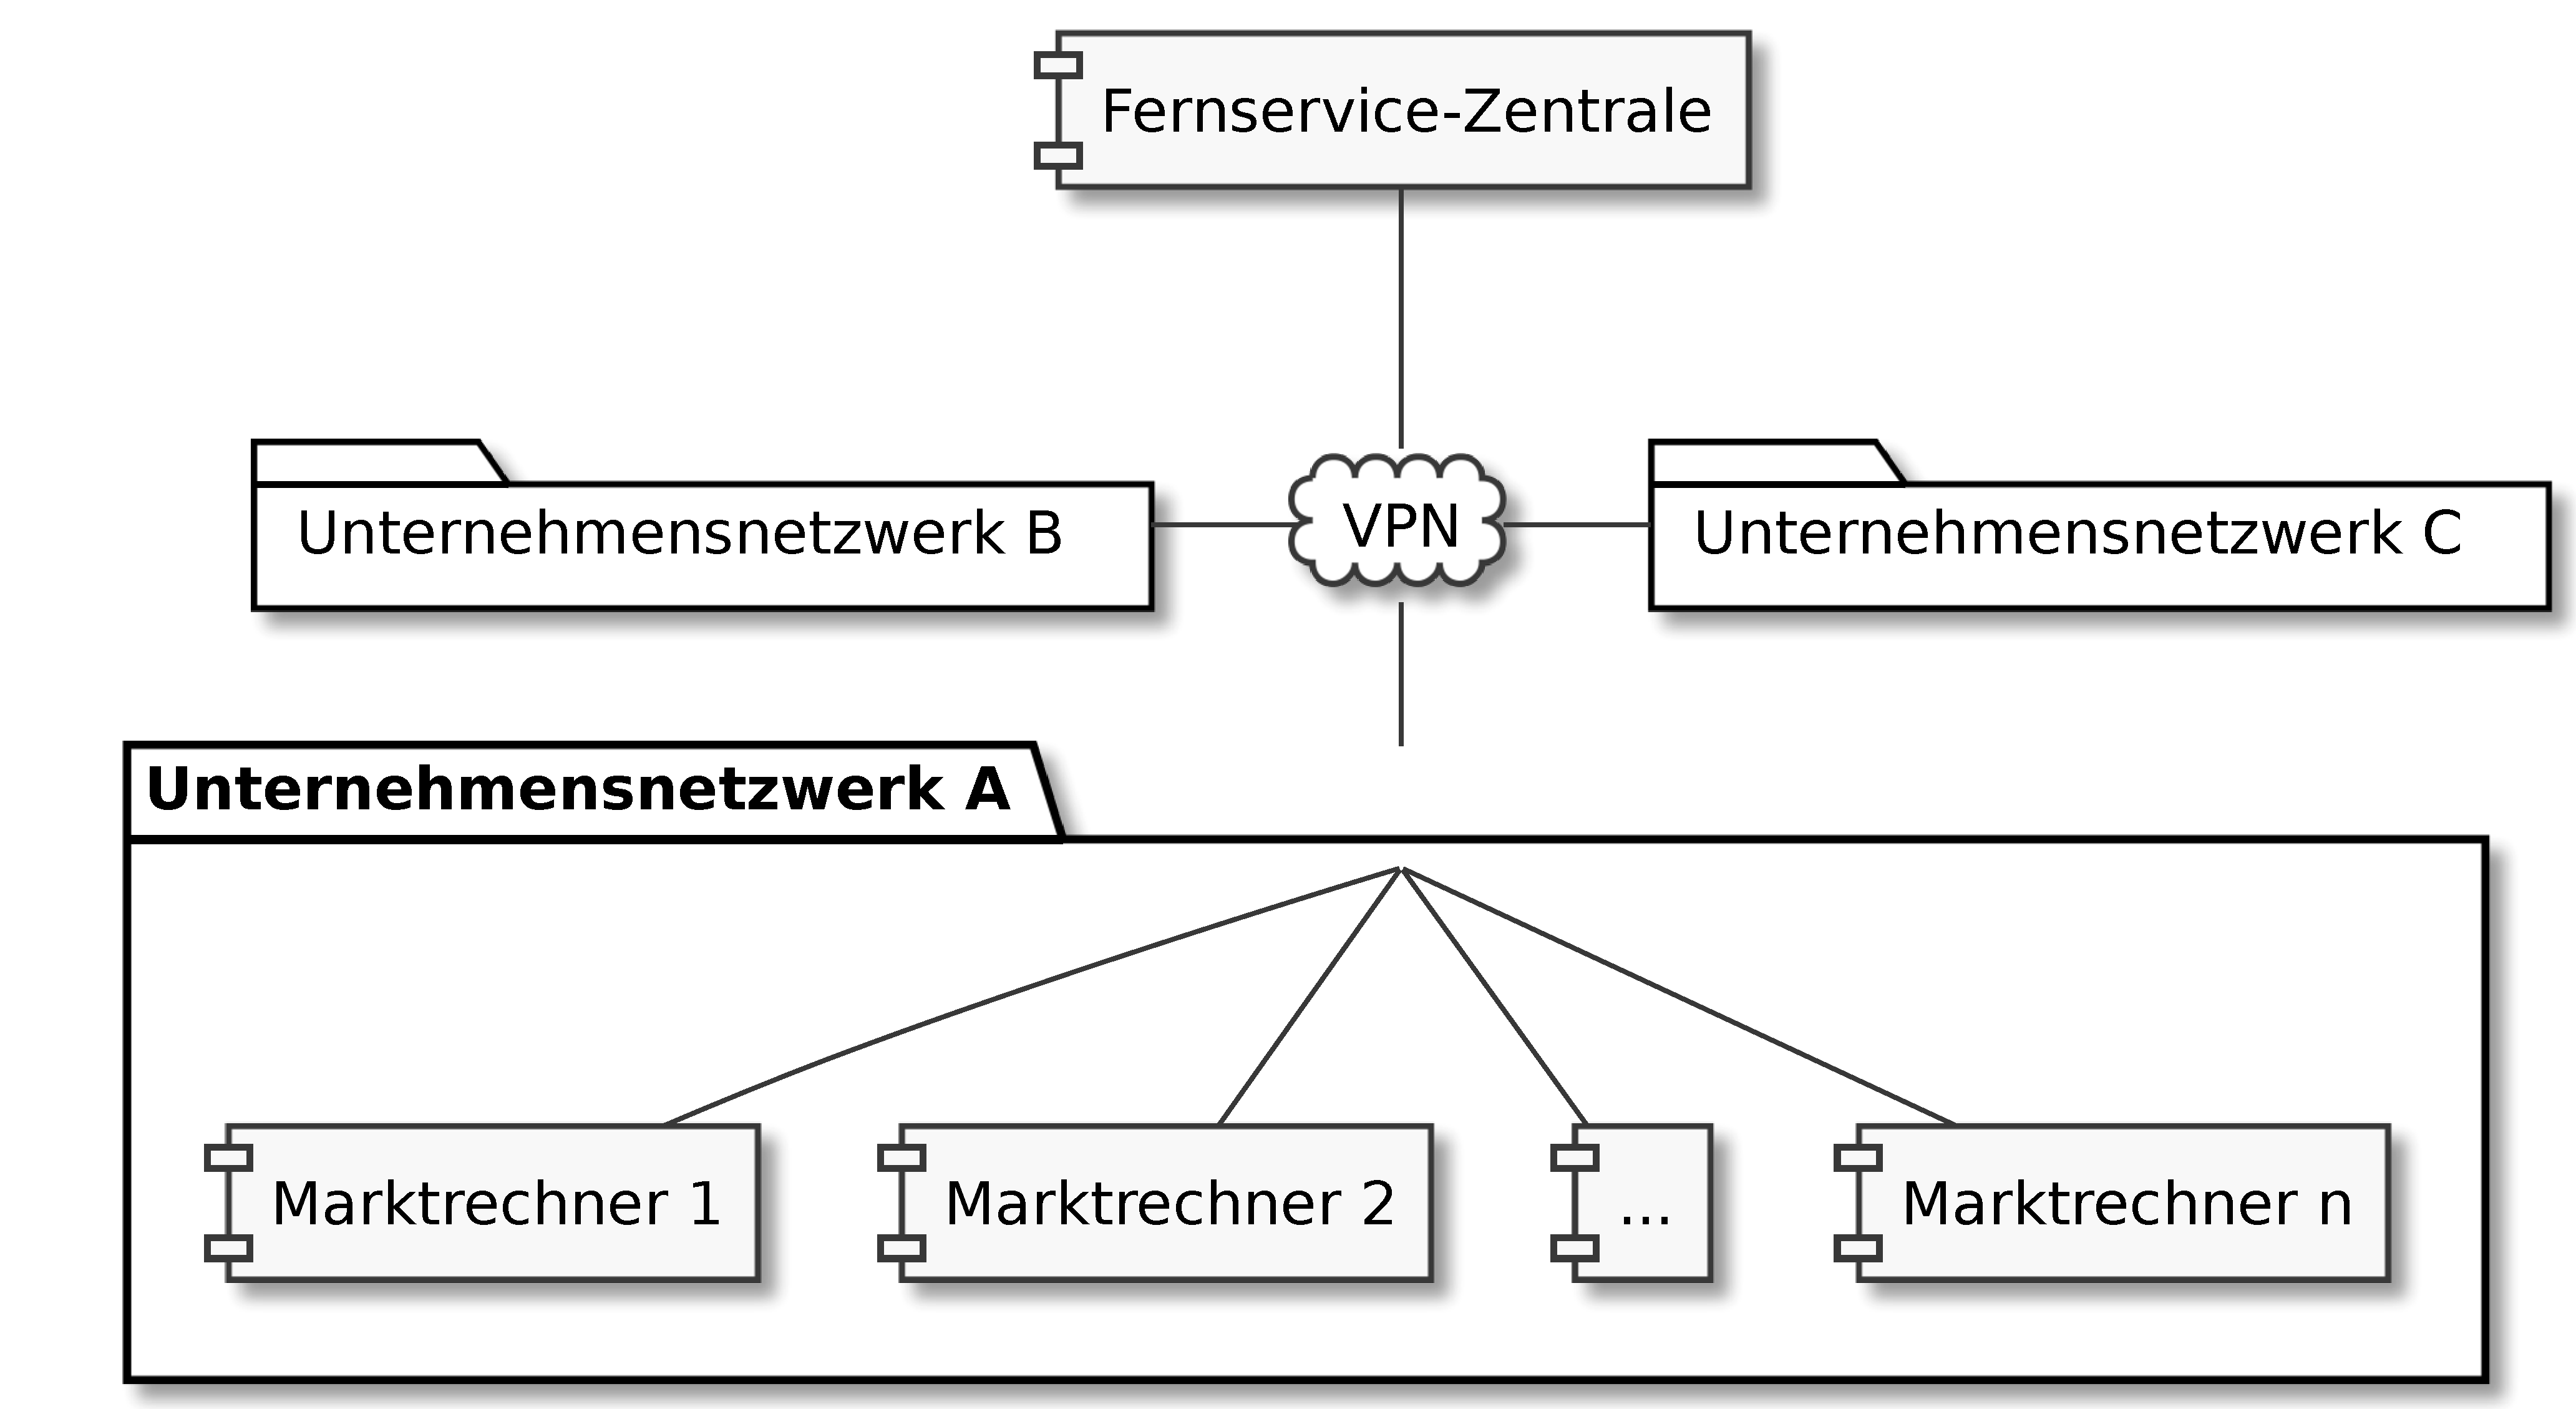
\includegraphics[scale=0.2]{images/problemfeld.pdf}
\caption{Aktuelle Vernetzung}
\label{fig:current_setup}
\end{figure}

Über VPN ist die Kommunikation von der Fernservice-Zentrale bis zum Unternehmensnetzwerk abgesichert. Im Lokal Area Network (LAN) des Unternehmens ist der gesamte Datenverkehr zu und von den Marktrechnern allerdings unverschlüsselt. Es gibt zwei Arten von Datenverkehr zum Marktrechner, zum Einen über das proprietäre Protokoll des Herstellers und zum Anderen über Webservices auf Basis von einfachen XML-RPCs. Ein Angreifer, mit Zugriff auf das LAN und Kenntnisse des Hersteller-Protokolls, hat die Möglichkeit den Datenverkehr zwischen Fernservice-Zentrale und Marktrechner mitzulesen. Was allerdings viel schwerer wiegt ist, dass ein solcher Angreifer über das Protokoll vollen lesenden und schreibenden Zugriff auf das System erhalten kann, da es keine geeignete Autorisierung und Authentifizierung gibt. Die Anzahl an Personen mit Wissen über das Hersteller-Protokoll ist zum Glück gering. Viel wahrscheinlicher ist ein Angreifer, mit Zugriff auf das LAN ohne Kenntnisse des Hersteller-Protokolls. Dieser kann den Datenverkehr zwischen XML-RPC und Fernservice-Zentrale mithören. Da in der XML die Daten interpretierbar aufbereitet wurden ist es ein leichtes diese Daten auszuwerten. Allerdings gibt es auch hier keine geeignete Autorisierung und Authentifizierung, wodurch der Angreifer statt mitzulesen, den XML-RPC selbst befragen kann. Dadurch erlangt er zwar keine vollen Zugriff auf das System, kann jedoch einige wichtige Schnittstellen auslesen und zum Teil auch neu konfigurieren. 

Neben diesen offensichtlichen Mängeln gibt es weitere. Sinnvolle, aussagekräftige Logs sind Hauptbestandteil eines guten Systems. Sinnvoll ist zum Beispiel das protokollieren des Systemzugriffs. Durch die ungeeigneten Sicherheitsmaßnahmen verliert das Zugriffslog jedoch komplett an Aussagekraft und ist damit wertlos. Ein weiterer Mangel ist, dass der Hersteller durch die existierende End-to-Site VPN-Verbindung keinen Zugriff auf seine Systeme erlangen kann. 


\section{Beschreibung der Problemsituation}

Das in Abschnitt~\ref{sec:problemfeld} geschilderte Problemfeld zeigt einige Mängel des aktuellen Systems auf. Im Folgenden werden die Probleme aufgezeigt, die gelöst werden sollen. Der Fokus dieser Arbeit liegt auf dem Fernzugriff, dennoch werden auch die Probleme des lokalen Zugriffes erfasst. Dadurch soll verhindert werden, dass der Fernzugriff unnötige Hindernisse für die lokale Umgebung schafft. 
Zunächst klären wir die Rollen im System, die Zugriffe auf Funktionen bekommen sollen. 

Die erste Rolle ist der Inbetriebnehmer. Er muss lokal, vor Ort die Anlage in Betrieb nehmen und soll dazu eine Offline-Konfiguration einspielen können, wodurch externe Systeme Zugriff auf die Anlage bekommen. Je nach Umgebung des Systems darf beziehungsweise muss der Inbetriebnehmer eine manuelle Konfigurationen vornehmen. Im Falle der Netzwerkkonnektivität muss dies ebenfalls vor Ort geschehen. Andere manuelle Konfigurationen, sowie die Kontrolle und Anpassung der Parameter und Einstellungen, zur Inbetriebnahme, ist durchaus aus der Ferne denkbar. Der Zugriff aus der Ferne würde ein Fernservice-Mitarbeiter vornehmen. Diese Rolle darf neben der bereits erwähnten Kontrolle und Anpassung von Parametern und Einstellungen das Alarm-Management durchführen. Dazu gehört sowohl die Konfiguration der Alarme, als auch deren Überwachung. Auch aus der Ferne arbeitet der System-Analyst. Dieser will relevante, vergleichbare Daten, wie etwa Temperatur-Daten oder Energie-Daten, auswerten, um mehrere Anlagen gegenüber zustellen. Das Marktpersonal ist daran interessiert eine Kontrolle der Parameter zur Warensicherheit durchzuführen und eine Dokumentationen der Waren-Temperaturen zu erhalten. Auch sollte dieses über Alarme informiert werden, um zum Beispiel Warenschaden zu verhindern. Die Rolle des Marktpersonal kann Zugriff vor Ort benötigen, aber auch der Zugriff aus der Firmenzentrale wäre denkbar.



::Rollen::

* Service-Mitarbeiter (Remote? -> Matthias)
* Inbetriebnehmer (Remote? -> Matthias)
* Fernservice-Mitarbeiter 
* System-Analyst
* Marktleiter/Marktpersonal
* Mitarbeiter des Herstellers
* Fremdsysteme

::Soziale Umgebung::

Remote (Fokus)
* Fernservice-Mitarbeiter will Zugriff auf die Anlage über LDSWin, REST, etc.
* Hersteller will Zugriff auf die Anlage SSH, LDSWin, etc.
* System-Analyst will Funktion zum Auslesen und Auswerten der Daten.

Locale (Für komplettes Bild)
* 


\section{Sichtweise der Verteidiger} 

\subsection{Wurzeldefinitionen}

\subsection{Konzeptionelles Modell}

\subsection{Vergleich mit der Realen Welt}

\section{Sichtweise der Angreifer}

\subsection{Wurzeldefinitionen}

\subsection{Konzeptionelles Modell}

\subsection{Vergleich mit der Realen Welt}



\chapter{Entwurf oder Design} \label{chap:design}

\begin{comment}
Im Rahmen des absolvierten Praktikums wurde eine neue Webservice-Schnittstelle geschrieben, welcher das weit verbreitete REST-Konzept für Webanwendungen zu Grunde liegt. Das RestGateway führt zur Zeit keine Authentifizierung und Autorisierung durch. Es wurde aber mit dem Hintergrund entwickelt, diese Funktionen zu integrieren.
\end{comment}

\chapter{Evaluation} \label{chap:evaluation}


%%%%%%%%%
% TABLE %
%%%%%%%%%
\begin{comment}
\begin{table}[htbp] % htbp ~ here, top, bottom, page
\centering
\begin{tabular}{|r|c|l|l|}
\hline
\textbf{Name} & \textbf{Adresse} & \textbf{Wohnort} & \textbf{Telefon} \\ 
\hline\hline
Susi Sinnlos & Eichenstrasse 5 & 12345 Unterstadt & 24927749242 \\
Horst Kurz & Schnellweg 17 & 42420 Rapid & 999 \\\hline
Jochanaan Leuchtentrager & Hochstraße zu & 666 Hell & 1-800-33845\\\hline
\end{tabular}
\caption{Adressliste}
\label{tab:meinetab}
\end{table}
\end{commit}

%%%%%%%%%
% ITEMS %
%%%%%%%%%
\begin{comment}
\begin{itemize}
\item Jede Tabelle, jedes Bild und jedes Listing ist ein Fließobjekt.
\item Zentrieren Sie Bilder und Tabellen.
\item Jedes Fließobjekt hat eine Bildunterschrift (Caption) mit
  einem Label und wird im Text passend referenziert.
\end{itemize}
\end{commit}

%%%%%%%%%%
% IMAGES %
%%%%%%%%%%

\begin{comment}
\begin{wrapfigure}{r}{6cm}
  \centering
  \includegraphics[width=4cm]{gnu}
  \caption{GNU-Logo~\cite{gnulogo,fal}}
  \label{fig:gnu}
\end{wrapfigure}
\end{comment}

\begin{comment}
\begin{figure}[htb]
\centering
\includegraphics[width=.6\textwidth]{zeichnung} % pdflatex ohne Endung
\caption{Die tolle Konzeptzeichnung}
\label{fig:tk}
\end{figure}
\end{comment}

\begin{comment}
\begin{figure}[htb]
\centering
\subfloat[Vektor]{\label{fig:vektor}
  \includegraphics[width=.3\textwidth]{zeichnung}}
\subfloat[JPG]{\label{fig:jpg}
  \includegraphics[width=.3\textwidth]{zeichnungjpg}}
\subfloat[PNG]{\label{fig:png}
  \includegraphics[width=.3\textwidth]{zeichnungpng}}
\caption{Die tolle Konzeptzeichnung in unterschiedlichen Formaten}
\label{fig:tk2}
\end{figure}
\end{comment}

\begin{comment}
\begin{figure}[htb]
\centering
\includegraphics[width=.4\textwidth]{zeichnungdraft} 
\caption{Die tolle Konzeptzeichnung als Draft}
\label{fig:tkdraft}
\end{figure}
\end{comment}

%%%%%%%%%%%
% LISTING %
%%%%%%%%%%%

\begin{comment}
\begin{listing}[htbp]
\lstset{basicstyle=\rmfamily, columns=[l]flexible, mathescape=true, showstringspaces=true, numbers=none, language=java}
\begin{lstlisting}
public static int ggt(int x, int y) {
    while (x != 0) {
      int h = x;
      x = y%x;
      y = h;
    }
    return y;
}
\end{lstlisting}
\caption{ggT --- Java}
\label{code:ggtjava}
\end{listing}
\end{comment}

\newpage

% Listen wenn überhaupt ans Ende und nicht an den Anfang.
% Meist ist das aber unnötig.
%\listoffigures % Liste der Abbildungen 
%\listoftables % Liste der Tabellen
% \newpage

\bibliographystyle{plain} % Literaturverzeichnis
\begin{btSect}{thesis} % mit bibtopic Quellen trennen
\section*{Literaturverzeichnis}
\btPrintCited
\end{btSect}
\begin{btSect}{online}
\section*{Online-Quellen}
\btPrintCited
\end{btSect}
% dann mit "bibtex thesis1" und "bibtex thesis2" arbeiten

\end{document}
;;; Local Variables:
;;; ispell-local-dictionary: "de_DE-neu"
;;; End:
